%%%%%%%%%%%%%%%%%%%%%%%%%%%%%%%%%%%%%%%%%%%%%%%%%%%%%%%%%%%%%%%%%%%%%%%%%%%%%%%%
% experiment.tex: Chapter describing the experiment
%%%%%%%%%%%%%%%%%%%%%%%%%%%%%%%%%%%%%%%%%%%%%%%%%%%%%%%%%%%%%%%%%%%%%%%%%%%%%%%%
\chapter{Experiment}
\label{experiment_chapter}
%%%%%%%%%%%%%%%%%%%%%%%%%%%%%%%%%%%%%%%%%%%%%%%%%%%%%%%%%%%%%%%%%%%%%%%%%%%%%%%%
%\subsection{Overview of the Compact Muon Solenoid and Large Hadron Collider}
The Compact Muon Solenoid (CMS) experiment was built to detect all Standard Model (SM) particles, and to
search for any non-SM interactions that produce SM particles, such as the interaction described in 
chapter ~\ref{wrBosonAndHeavyNu}.  Two high-energy proton beams collided at the geometric center of
the CMS experiment, and interactions between colliding protons were recorded.

Interactions between protons were identified by the detection of:
\begin{itemize}
	\item one or more energetic charged leptons (electron, muon, tau or their anti-particles)
	\item one or more energetic photons
	\item one or more energetic hadronic jets
	\item one or more energetic neutrinos\footnote{the presence of neutrinos is inferred from the vector sum of momentum of all charged leptons, photons and hadronic jets detected in a collision event.}
	\item combinations thereof
\end{itemize}
Particles produced by proton-proton (pp) interactions were detected using a 3.8$\unit{T}$ magnet and four CMS 
sub-detector systems.  The full strength magnetic field volume enveloped the region where pp interactions occurred, and three of the four 
sub-detector systems used in particle detection.  As shown in Figure \ref{fig:layersOfCMS}, surrounding the pp interaction
region was the silicon tracker in which charged particles were first detected.  As charged particles traversed
the tracker, mobile electron-hole pairs were ionized in several layers of silicon along the trajectories of charged
particles.  Charged particles were detected in the tracker by measuring the charge ionized in all silicon layers.

\begin{figure}[h]
	\centering
	
\includegraphics[width=0.6\textwidth]{figures/missingImage.png}
	\caption{Cross section view of the entire CMS detector in a plane perpendicular to the beam axis.  Closest to the
	proton-proton interaction region is the silicon tracker, followed by the Electromagnetic Calorimeter, then the Hadronic 
Calorimeter, and the magnet.  Outside the magnet are the muon detectors.}
	\label{fig:layersOfCMS}
\end{figure}


Surrounding the silicon tracker was the second of three sub-detector systems enclosed in the full strength magnetic field, the
lead-tungstate crystal (PbWO$_{4}$) Electromagnetic Calorimeter (ECAL).  The ECAL was an absorption calorimeter that
detected photons produced by pp interactions, and distinguished electrons and positrons from other charged 
particles detected by the tracker.  Electrons, positrons and photons interacted with lead-tungstate nuclei 
through bremsstrahlung and electron-positron pair production processes, and produced showers of lower energy
electrons and positrons.  Through Coulomb interactions, these lower energy particles excited atomic electrons
of lead-tungstate nuclei to higher energy, meta-stable bound states.  When these atomic electrons transitioned
back to the ground state, visible light photons were produced.  High energy photons, electrons and positrons 
produced by pp interactions were detected by measuring the visible light produced in lead-tungstate crystals.

Wrapped around the ECAL was the last of three sub-detector systems enclosed in the full strength magnetic field, the brass and 
plastic scintillator Hadronic Calorimeter (HCAL).  Built from alternating layers of brass absorber and scintillating
plastic tiles, the HCAL was a sampling calorimeter that detected charged and neutral hadrons.  Charged and 
neutral hadrons that travelled through the tracker and the ECAL interacted with bound nucleons in brass absorber layers
through diffractive and inelastic scattering processes.  Scattering events produced showers of lower energy hadrons, which
travel through nearby scintillating plastic tiles.  Interactions between low energy hadrons and molecules in
the plastic excited the molecules to meta-stable states.  When excited molecules transitioned back to the ground 
state, visible light photons were emitted.  High energy charged and neutral hadrons produced by pp interactions 
were detected by measuring the visible light produced in scintillating plastic tiles.

Outside the HCAL was the 3.8$\unit{T}$ magnet.  The magnetic field was generated by running a current of 
$\lesssim$18 thousand amps through superconducting wire wound into a solenoid.  The wire, made from a niobium alloy, was 
cooled to a superconducting state using a liquid helium adsorption refrigerator and liquid nitrogen precooling 
system.  The cryogenic system and magnet were supported by a separate structure built from iron, steel and titanium.  The
large volume of material linked to the magnet and support systems provided a barrier through which only muons 
could penetrate.

Surrounding the magnet was the fourth sub-detector system used to detect particles, the muon detectors, which resided 
in the magnet return yoke where the magnetic field strength was 1$\unit{T}$.  Three 
different technologies - drift tubes (DT) in the lowest radiation regions, cathode strip chambers (CSC) in higher 
radiation regions, and resistive plate chambers (RPC) in all regions - were used to detect muons.  In detectors of all 
three technologies, muons travelled through pressurized gas chambers and ionized electrons from the gas along their 
trajectories.  Within the chambers, electric fields accelerated the ionized electrons towards conducting wires.  Muons 
were detected by measuring the charge collected by conducting wires.

Due to the enormous rate of pp collisions in which only elastic or diffractive scattering occurred, a two tiered trigger 
system was used to select events where energetic charged leptons, hadronic jets, photons, neutrinos or combinations 
thereof were detected.  The first tier of the trigger system processed information from the ECAL, the HCAL and the muon 
detectors in small regions where high energy particles were detected.  Regions in which the detected energy exceeded 
a preset threshold were then processed by the second tier of the trigger system.  In the second tier, reconstruction software 
was run in selected regions to identify charged leptons, photons, jets and neutrinos.  If a pp collision event produced one 
or more of these reconstructed particles that passed quality and energy cuts defined in the second tier, then all data 
from all four sub-detector systems for that event was read out and written to disk.

The accelerator which collided the proton beams, the coordinate system used to characterize the kinematics of detected 
particles, the silicon tracker, both calorimeters, the muon detectors and the trigger system are discussed in this chapter.

\section{The Large Hadron Collider}
\label{sec:lhcDescription}
Situated near Geneva, Switzerland and spanning the French-Swiss border, the CERN Large Hadron Collider (LHC) accelerated 
two counter-rotating proton beams in a 27 km circular tunnel (CITE) up to an energy of 6.5 TeV in 2015.  At several points along the tunnel 
the two beams collided, and surrounding one of these points the CMS experiment was built.

Several accelerator stages were used to create a proton beam in the LHC.  Summarized in Figure \ref{fig:accelComplex} (CITE), each 
proton beam began as isolated proton bunches ionized from hydrogen gas.  Proton bunches were first accelerated by a linear 
accelerator, LINAC 2, and were then injected into the circular Proton Synchrotron (PS) accelerator.  Protons were accelerated 
to an energy of 26 GeV by the PS, and then were injected into the circular Super Proton Synchrotron (SPS) accelerator.  
The SPS accelerated proton bunches to an energy of 450 GeV, which were subsequently injected into the LHC.  Once the SPS 
injected the desired number of proton bunches to fill two beams, the LHC accelerated both beams to the desired energy, 
and focused the beams to increase the rate of pp collisions.  In 2015 each beam was accelerated to an energy of 6.5 TeV, and 
contained as many as 2300 proton bunches.

In the LHC tunnel, superconducting radio-frequency (RF) cavities accelerated proton bunches, and magnets steered and 
focused the beams towards the collision point at the heart of CMS.  Sixteen RF cavities (8 per beam) accelerated proton 
bunches to an energy of 6.5 TeV, and also served as a control system in which protons in any bunch moving too quickly 
were slowed, while protons moving too slowly experienced greater acceleration.  Dipole, quadrupole and higher order 
magnets operated at magnetic field strengths up to 8$\unit{T}$ steered the beams around the LHC, and focused them 
on the collision point inside CMS to increase the rate of pp interactions.

DISCUSS INST AND INTEGRATED LUMI, CONNECT TO 2015 COLLISION DATA AND SEARCH FOR LOW XSXN WR PRODUCTION

\section{The CMS Coordinate System and Kinematic Variables}
\label{sec:coordinateSystemAndKinematicVars}
The coordinate system and variables used to characterize the kinematics of detected particles were defined in 
the following way.  The right-handed coordinate system was defined with the $z$ axis pointed in the direction 
of the counter-clockwise rotating beam, the $y$ axis pointed up towards the surface, and the $x$ axis pointed towards 
the center of the LHC ring.  In this coordinate system particle trajectories were measured using two angular 
variables, $\phi$ and $\eta$, that were defined in terms of angles in two coordinate planes.  $\phi$ was defined 
as the angle in the $x-y$ plane, and took values between 0 and $2\pi$.  The angle $\theta$ in the $y-z$ plane, 
which was 0 ($\frac{\pi}{2}$) when pointing along the $z$ ($y$) axis, was transformed into pseudorapidity 
$\eta$ through the following function:

\begin{equation*}
	\eta \equiv -\ln{\tan{\frac{\theta}{2}}}
\end{equation*}

Pseudorapidity of 0 was the $y$ axis, and pseudorapidity of $\infty$ was the $z$ axis.
An equivalent definition of pseudorapidity in terms of the energy E and longitudinal 
momentum $p_{z}$ of a particle in the massless particle limit was:

\begin{equation*}
	\eta \equiv \frac{1}{2}\ln{\frac{E+$p_{z}$}{E-$p_{z}$}}
\end{equation*}

Pseudorapidity was used to describe particle trajectories instead of the angle $\theta$ for several reasons.  Particles 
produced by pp interactions were usually boosted along the $z$ axis, but the degree of boost was never well 
defined because the momenta of the interacting partons could never be measured.  This boost affected the 
trajectories of particles in $\theta$, but did not affect particle trajectories measured in $\eta$.  In 
addition, the particles that caused radiation damage in CMS sub-detector systems were produced at 
a rate that scaled linearly with $\eta$.  Thus, in discussions about topics where radiation damage 
or particle isolation played a role, ideas could be more clearly articulated using $\eta$.

The main variables used to quantify the energy of a detected particle were transverse energy 
$E_{T} \equiv E/\cosh{\eta}$ and transverse momentum $p_{T} \equiv |p|/\cosh{\eta}$, while the distance between 
a particle and another point in the $(\eta, \phi)$ space was measured as $\Delta R \equiv \sqrt{\eta^{2} + \phi^{2}}$.  
Transverse momentum, the component of momentum perpendicular to the proton beam axis, and transverse energy, the 
analogous form of energy, were used because both were insensitive to the unknown momenta of the interacting partons.  
Explained in later chapters, the distance $\Delta R$ was measured between the trajectory of one particle 
and another point in the $(\eta, \phi)$ space, which often was the trajectory of another particle.

\section{The Silicon Tracker}
\label{sec:siTrackerDescription}
Built from separate silicon pixel and silicon strip trackers, the silicon tracker detected charged particles  
and measured their momenta, and identified interaction vertices where charged particles were produced.  Closest 
to the beam axis was the pixel tracker, which used small silicon pixels to pinpoint pp interaction vertices 
with $\mu$m precision.  Surrounding the pixel tracker were larger silicon strip detectors that measured the 
momenta of charged particles.  Charged particles produced within the tracker acceptance of $|\eta| < 2.5$ ionized 
charge in the silicon pixel and strip trackers, and the measurement of this charge formed the basis for all tracker 
measurements.

Charged particles produced by pp interactions ionized charge in every silicon tracker cell they hit, and attached 
to each cell was a charge readout module.  Using a $\lesssim$100 V electric potential, each readout module created 
an electric field along the surface of its silicon cell that swept ionized charge into a charge collector.  The 
orientation of the silicon cells relative to the magnetic field direction was chosen so that the beneficial effect 
of the magnetic field on charge collection was maximized.

The pixel tracker was built from several layers of the pixel 

To 
accommodate greater particle fluxes and radiation damage at increasing $|\eta|$, the pixel and strip 
detectors were split into barrel ($|\eta| < 1.2$) and endcap ($|\eta| \geq 1.2$) sections.  .


\section{The Electromagnetic Calorimeter}
\label{sec:ecalDescription}

%After traversing the tracker, electrons and positrons interacted with 
%lead-tungstate nuclei through the bremsstrahlung process and produced gamma rays.  Gamma rays then interacted 
%with lead-tungstate nuclei and were converted into electron-positron pairs.  For every electron or positron
%that impinged on the ECAL, this two step cycle of bremsstrahlung followed by pair conversion repeated many 
%times, and a shower of lower energy electrons and positrons was made.  Energetic photons that impinged on
%the ECAL were first converted into an energetic electron-positron pair, then the same two step cycle ensued
%and produced showers of lower energy electrons and positrons.  These .



\section{The Hadronic Calorimeter}
\label{sec:hcalDescription}


\section{The Muon Detectors}
\label{sec:muonDetectorsDescription}

\section{The Trigger System}
\label{sec:triggerDescription}




The Compact Muon Solenoid (CMS) was built to detect new particles produced by proton-proton (pp) collisions 
in the Large Hadron Collider (LHC).  Situated underground near the French-Swiss border and
operated by the European Organization for Nuclear Research (CERN), the LHC collided protons at
$\sqrt{s} = 13 TeV$ center-of-mass energy to search for new particles like the WR boson discussed 
in Sec. ~\ref{wrBosonAndHeavyNu}.  Evidence of the WR boson was sought in pp collision events that
produced Standard Model (SM) leptons and hadronic jets.  The CMS detector used to identify leptons and
jets is described herein.

The

%use this lumi info in the trigger section.  it is not relevant for the detection of leptons and jets
%why are high lumi and energy needed
The LHC was built to discover new physics mediated by heavy particles which are weakly coupled to Standard Model (SM)
leptons, hadrons and bosons.  To produce heavy, weakly interacting particles, like a $2.0 TeV$ mass right handed W ($W_{R}$) boson
with production cross section 5 fb, at a rate sufficient for detection, average instantaneous luminosities of
$10^{33} \frac{1}{cm^{2}s}$ are needed.  At such luminosities, other more abundant or lower energy processes will occur
at a significant rate, as shown in Figure \ref{fig:smProductionXsxns}.

Of all processes created by collisions in the LHC, low energy, inelastic QCD interactions occur at the highest rate, of the order
$10^{8}$ events per second at $10^{33} \frac{1}{cm^{2}s}$.  Contributions from these events to new physics searches are mitigated by vetoing
on large groups of particles collinear with the beam line, or requiring the presence of leptons or photons.  However, these
requirements are not sufficient to suppress leptonic backgrounds created by the production and decay of heavy quarks, and QCD multijet
events in which a jet is incorrectly reconstructed as a lepton due to energetic neutral pions in the jet.  Such high energy QCD multijet
and heavy quark decay events occur at a rate of $10^{5}$ events per second at $10^{33} \frac{1}{cm^{2}s}$.  These event rates dwarf
the rate at which entire events can be read out of CMS and saved to disk, approximately $10^{3}$ events per second.  The tools, generally
called triggers, used to select and save collision events at approximately $10^{3}$ Hz will be discussed later.

\begin{figure}[h]
	\centering
	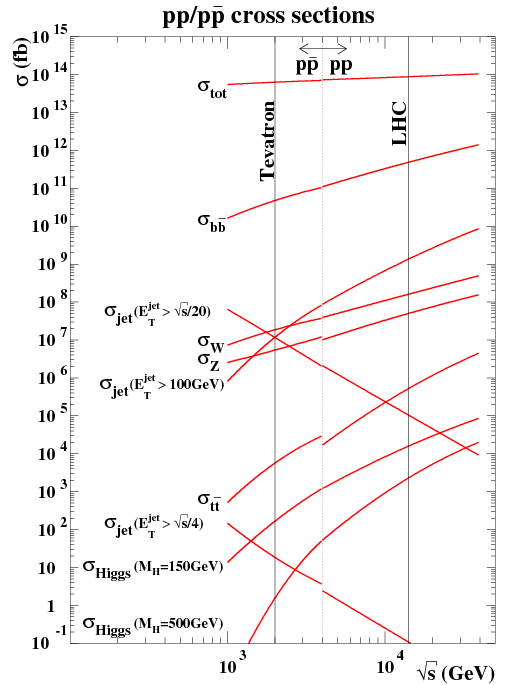
\includegraphics[width=0.6\textwidth]{figures/lhc_and_tevatron_cross_sections_2006.png}
	\caption{Production cross sections at the LHC and Tevatron as a function of center of mass energy. \cite{}}
	\label{fig:smProductionXsxns}
\end{figure}


%Operations
The LHC started operations with collisions at a lower center of mass energy and lower instantaneous luminosity than design.  In 2015 the center of mass
energy was increased to 13 TeV, and the luminosity was increased closer to the design level.  The 2015 data taking period was split into two portions - from the start
of 2015 collisions until August the time separation between consecutive proton bunches in each beam was 50 ns.  After August, the bunch
separation decreased to 25 ns to increase the instantaneous luminosity, and proton proton collisions continued until November.  From August until November, instantaneous 
luminosities reached $5x10^{33} \frac{1}{cm^{2}s}$, but problems with the CMS
magnet cooling system limited the amount of data collected to 2.6 $fb^{-1}$.  Decreasing the bunch spacing increased the sensitivity of every new physics search, but
came with the cost of more proton proton interactions in every bunch collision, or pileup.  At 13 TeV the total inelastic cross section is approximately 70 mb \cite{Haevermaet}, 
so for instantaneous luminosities between $3-5x10^{33} \frac{1}{cm^{2}s}$ in 25 ns running the expected pileup per bunch crossing is $8-13$, which is consistent with
the pileup observed in 25 ns collision data.  Pileup increases the complexity of events$\footnote{15 inelastic pp collisions yield a total flux of particles similar to one top antitop quark pair event}$, and makes event reconstruction and offline analysis more challenging.


\subsection{Compact Muon Solenoid Detector Overview}
\begin{itemize}
	\item trigger description, followed by particle flow event reconstruction
\end{itemize}
The Compact Muon Solenoid (CMS) experiment is designed to search for signs of new physics at the high energy and luminosity regime probed by the LHC.  The LHC was built
as a discovery machine, so particular attention has been paid to searches for physics beyond the SM (BSM), such as supersymmetry and extensions of the SM.

The The CMS detector approximates a cylinder in shape, with a length of 22 meters, outer radius of 7 meters, and weight of 14500 tons.  It is divided into a central barrel region ($|\eta| < 1.4$)
in which separate subdetectors are arranged as concentric cylindrical shells at increasing radii from the beam axis, and a forward endcap region ($|\eta| > 1.4$) 
in which subdetectors are arranged as layers stacked along the beam axis.  Illustrated in Figure \ref{fig:cmsDetectorComponentView}, the CMS subdetectors have complete 2$\pi$ radian coverage in
$\phi$, and hermetic calorimeter coverage from $-5 \leq \eta \leq 5$ ($-179^{\circ} \leq \theta \leq 0.77^{\circ}$) with respect to the beam axis.  Complete detector
coverage over this large angular range allows precise measurements to be made of missing energy, and the mass of yet-undiscovered light and heavy particles.

\begin{figure}[h]
	\centering
	
\includegraphics[width=0.6\textwidth]{figures/missingImage.png}
	\caption{The CMS detector with the coordinate system shown   .  The x axis points towards...}
	\label{fig:cmsDetectorComponentView}
\end{figure}


Starting at the interaction point and going radially outward, the first subdetector encountered by particles produced in collisions is the silicon tracker.
The tracker consists of silicon pixel detectors surrounded by silicon strip detectors, all of which are immersed in a 3.8 Tesla magnetic field produced by a superconducting solenoid.
Both detectors are only sensitive to charged particles, and facilitate precise measurements of charged particle momenta
and the positions of interaction vertices by measuring the curvature of charged particle tracks which have $|\eta| \leq 2.5$.

Particles which exit the tracker with sufficient momentum to travel approximately 1.0 meter radially away from the interaction point will reach the
electromagnetic calorimeter (ECAL).  ECAL consists of approximately 76000 lead tungstate crystals which, like the tracker, are sit in a 3.8 Tesla
magnetic field.  The radiation hardness and fast scintillation time of lead tungstate were key factors in chosing to build ECAL out of it.
ECAL was designed to measure the energy, time, position and shower shape of electrons and photons with $|\eta| \leq 3.0$ by measuring scintillation
light produced by lead tungstate in electron and photon showers.

Particles which traverse ECAL with sufficient momentum to continue moving away from the interaction point hit the hadronic calorimeter (HCAL).  Built
from alternating layers of metal and scintillating plastic tiles, HCAL was designed to measure the energy of charged and neutral
hadrons, and to provide structural support to all of CMS.  Energetic hadrons produce showers of lower energy particles in metal layers, and the
showers which reach nearby scintillating tiles produce scintillation light.
HCAL extends out to $|\eta| = 3.0$, is enveloped by the 3.8 Tesla magnetic field, and
is complimented by a forward hadron calorimeter (HF) which extends the calorimetry coverage out to $|\eta| = 5.0$.  Due to the high radiation
environment in its vicinity, HF is built from radiation hard steel blocks laced with radiation hard quartz fibers.  Charged particles which travel
through HF produce Cherenkov light in the quartz fibers; from the Cherenkov light an energy measurement is extracted.

Surrounding HCAL is the CMS magnet.  It produces a 3.8 Tesla magnetic field from superconducting niobium titanate wire wound into a solenoid, and
carries more than 10000 amps of current during normal operation.

Particles which pass through HCAL and the magnet encounter the last CMS subdetector, designed to measure the energy of muons.  The muon
detectors consist of three technologies - drift tubes (DT) and resistive plate chambers (RPC) which cover out to $|\eta| \leq 1.3$, while cathode
strip chambers (CSC) and RPCs which cover $1.3 \leq |\eta| \leq 2.4$, with some overlap near $|\eta| = 1.3$.  All three technologies measure the amount
of charge ionized in a gas when a muon traverses an enclosed volume filled with gas, and convert this charge into an energy.

All CMS subdetectors are utilized in particle flow (PF) reconstruction and event triggering.  In. 

\subsection{Track and vertex reconstruction}

\subsection{Muon Reconstruction and Identification}
\begin{itemize}
	\item importance of muons, challenges with reco and energy measurements
	\item muon detector technologies
	\item muon reconstruction algorithms
	\item challenge with pT measurement of high pT muons
	\item explain TuneP algorithm and show performance plots
	\item explain ID variables, isHighPt ID and show performance plots
	\item explain usefulness of muon isolation (reject muons from QCD) and how it is calculated
	\item muon L1 and HLT: design and performance plots
\end{itemize}

\subsection{Electron Reconstruction and Identification}
\begin{itemize}
	\item importance of electrons, challenges with reco and energy measurements
	\item ECAL
	\item electron reconstruction algorithms
	\item challenge with pT measurement of high pT muons
	\item explain TuneP algorithm and show performance plots
	\item explain ID variables, HEEP ID and show performance plots
	\item explain usefulness of electron isolation (reject eles from QCD) and how it is calculated
	\item electron L1 and HLT: design and performance plots
\end{itemize}



\subsection{Particle Flow and Jet Reconstruction}



